Verifichiamo la bontà della regressione eseguita nel paragrafo precedente tramite il test del chi quadro.
Il valor atteso $\chi^2_{\text{teo}}$ del test è uguale al numero di gradi di libertà del sistema. Nel nostro caso
esso vale $\chi^2_{\text{teo}} = N - 2 = 8$ poiché dal fit sono stati calcolati 2 parametri. Poiché
il numero di gradi di libertà è basso, abbiamo deciso di adottare un intervallo di confidenza del tipo $[0, h]$,
dove $h$ è il valor critico del chi quadro. Scelta la probabilità di falso allarme del 5 \%, dalla distribuzione
del chi quadro si può calcolare $h = 15.5$. Quindi l'intervallo di confidenza è [0, 15.5]. 

Utilizzando i valori $A$ e $b$ trovati precedentemente, calcoliamo l'espressione

\begin{equation}
    \chi^2_{\text{oss}} = \sum_{i=1}^\mathcal{N} \frac{(Y_i - A - bX_i)^2}{(\delta Y_i^{\text{tot}})^2} = 29.4
\end{equation}
%
che è chiaramente al di fuori dell'intervallo di confidenza.

\begin{SCfigure}[][t]
    \centering
    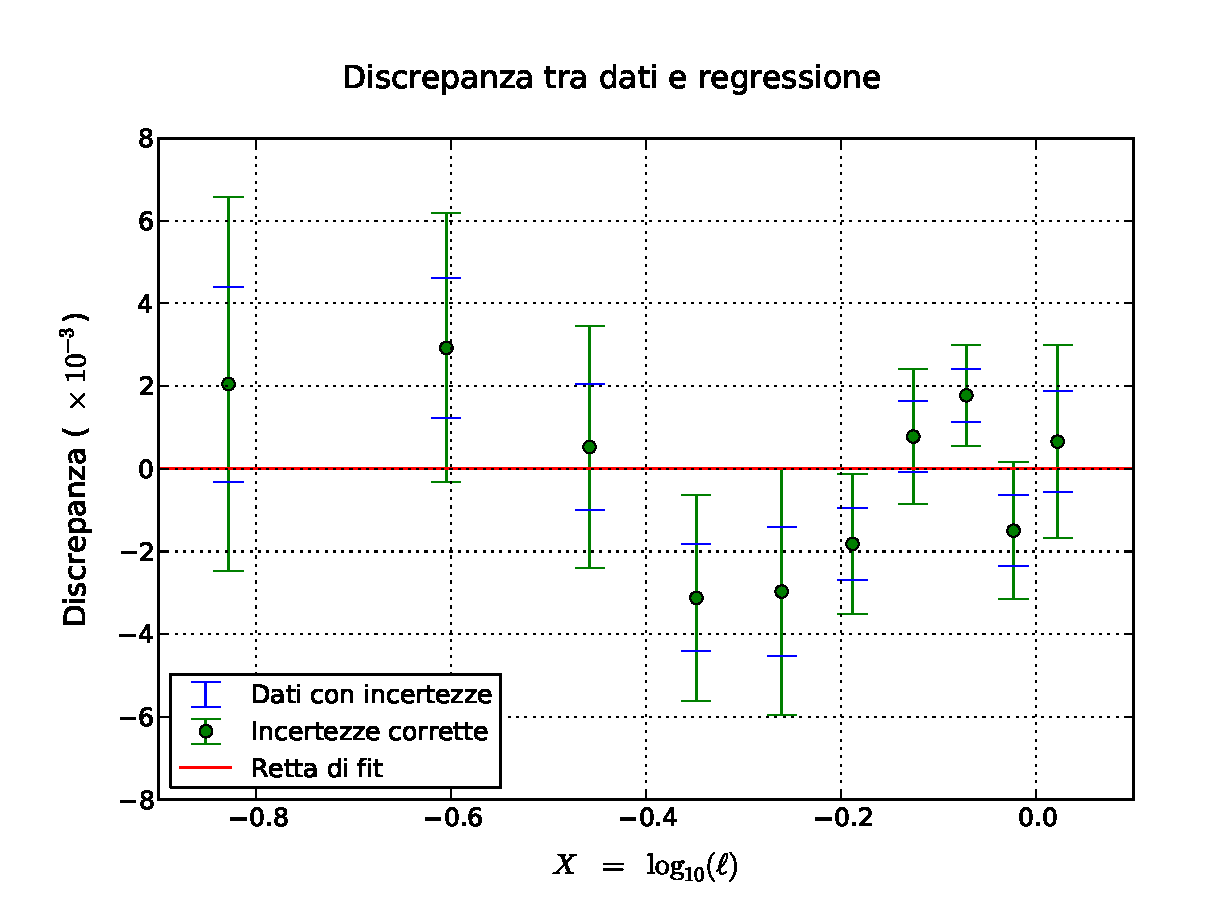
\includegraphics[width=115mm]{immagini/l_discrepanza.pdf}
    \caption{Il grafico mostra la discrepanza tra dati sperimentali e retta di fit, ottenuta con la formula $Y_i - A - bX_i$.
        Le barre di errore blu mostrano il valore delle incertezze prima della correzione, mentre quelle verdi mostrano gli errori
        corretti. Si nota che le barre d'errore prima della correzione erano piccole, e ciò ha causato un alto
        valore del $\chi^2$, e che la correzione è abbastanza cospicua. Non sembra visibile alcun andamento residuo nei dati.
        In entrambi gli assi sono riportati numeri puri.}
    \label{fig:l_discrepanza}
\end{SCfigure}

A questo punto abbiamo controllato che non ci fossero punti sperimentali che contribuissero significativamente
al chi quadro. Il grafico in Figura \ref{fig:l_discrepanza} mostra la discrepanza tra dati e retta di fit,
ovvero la differenza $Y_i - A - bX_i$. In questo modo si possono visualizzare le incertezze e si può verificare
in maniera approssimata la stima del chi quadro. Non ci sono punti che influenzano da soli in modo significativo
il valore del chi quadro (si osservino le barre d'errore blu), al contrario risulta chiaro che l'alto valore di $\chi^2$
è dovuto a più punti.

Segue che probabilmente questa incompatibilità è dovuta al fatto che l'incertezza sui periodi è stata sottostimata.
Questo può essere dovuto a diversi fattori, primo fra tutti l'errore sistematico dovuto all'operatore. Dobbiamo
far notare che le misure, in questo esperimento, sono state rilevate da un singolo operatore che può aver introdotto
un errore sistematico. Supponiamo che
l'errore dovuto allo sperimentatore sia la causa del valore eccessivo del chi quadro. Procederemo ora a correggere le incertezze,
e successivamente verificheremo se la correzione eseguita è accettabile e convincente.

Aggiustiamo quindi le incertezze per far tornare il chi quadro.  Poiché le incertezze sono diverse per ciascun punto,
moltiplichiamo ogni incertezza $\delta Y_i^{\text{tot}}$ per un fattore $q$ e determiniamo per quale valore di $q$
il chi quadro diventa uguale al suo valore atteso

\begin{equation}
    \chi^2 = \sum_{i=1}^\mathcal{N} \frac{(Y_i - A - bX_i)^2}{(q\, \delta Y_i^{\text{tot}})^2} = N - 2 = 8
\end{equation}
%
Poiché $q$ è uguale per tutti i valori di $\delta Y_i^{\text{tot}}$, si può portare fuori dal segno di sommatoria.
Successivamente, mediante passaggi algebrici elementari, si arriva al seguente risultato

\begin{equation}
    q^2 = \frac{1}{8} \sum_{i=1}^\mathcal{N} \frac{(Y_i - A - bX_i)^2}{(\delta Y_i^{\text{tot}})^2} = 3.68 \qquad \text{ovvero} \qquad q = 1.92
\end{equation}

Abbiamo quindi calcolato che, affinchè il chi quadro diventi uguale al suo valor atteso, è necessario moltiplicare
le incertezze per un fattore $q \simeq 1.9$. Le incertezze vanno quindi aumentate del 90 \% circa.

L'aggiutamento da eseguire è quindi abbastanza elevato. Poiché la correzione si riferisce al valore $\delta Y_i^{\text{tot}}$,
per verificare se è plausibile una correzione di questa entità, proviamo a risalire alla correzione da fare sul valore di lettura
dello strumento, per vedere se può trattarsi di un sistematico dovuto all'operatore.

Poiché sappiamo che $\mathcal{T} = 10^Y$, con la propagazione dell'incertezza otteniamo:

\begin{equation}
    \delta \mathcal{T}\ped{corr} = \frac{10^Y}{\log_{10}(e)} \delta Y\ped{corr}
\end{equation}
%
dove con $\delta \mathcal{T}\ped{corr}$ e $\delta Y\ped{corr}$ indichiamo rispettivamente le incertezze corrette sul periodo e sulle $Y$.
Le nuove incertezze sul periodo $\delta \mathcal{T}\ped{corr}$ si riferiscono alle medie di dieci misure, per cui,
per ottenere l'incertezza corretta per ogni misura occorre moltiplicare questa incertezza per $\sqrt{N}$ dove $N = 10$
indica il numero di misure di periodi effettuate per ogni lunghezza. Inoltre ogni singola misura è stata ottenuta dividendo per 5 il valore
di lettura del cronometro, per cui occorre moltiplicare per cinque l'errore. L'incertezza corretta sul valore di lettura del cronometro
vale quindi

\begin{equation}
    \delta \mathcal{T}\ped{lettura} = 5\, \sqrt{10}\: \delta \mathcal{T}\ped{corr}
\end{equation}

Le incertezze così ottenute, riferite al valore di lettura del cronometro, variano da un minimo di circa \SI{0.08}{\second} ad un massimo
di circa \SI{0.18}{\second}. Questi valori sono troppo alti per essere dovuti solamente all'operatore. Se sembra infatti convincente
che un errore sistematico dovuto all'operatore possa avere un entità di qualche centesimo di secondo (fino ad un decimo), è
molto più difficile che si arrivi ad un errore di \SI{0.18}{\second}. Dobbiamo quindi dedurre che abbiamo un errore sistematico
sconosciuto di cui non sappiamo la causa. Tuttavia arrivati a questo punto proseguiamo comunque con il resto della relazione, dando
per buone le incertezze a posteriori, tenendo comunque presente che c'è una causa di errore ignota.

\subsubsection{Conclusione della regressione}
\label{l_end_fit}

Poiché sono state modificate le incertezze, prima di calcolare i valori definitivi di $a$ e $b$ e concludere l'esperimento,
è necessario ripetere la procedura di fit per calcolare le nuove incertezze $\delta A$ e $\delta b$

Occorre quindi minimizzare la funzione

\begin{equation}
    \sum_{i=1}^\mathcal{N} \frac{(Y_i - A - bX_i)^2}{(b\,\delta Y_i^{\text{tot}})^2}
    \label{eq:l_min_quad_2}
\end{equation}

Dalla minimizzazione si ricavano i valori

\begin{equation*}
    A = 0.3024 \qquad \qquad b = 0.499
\end{equation*}
%
che sono, correttamente, identici a quelli ricavati nel paragrafo \ref{l_regressione}.
Infatti la funzione (\ref{eq:l_min_quad_2}) differisce da (\ref{eq:min_quad}) solo per una costante
moltiplicativa e conserva inalterati il punto di minimo.

Le incertezze su $A$ e $b$ calcolate partendo dai valori aggiustati degli errori $\delta Y_i^{\text{tot}}$
valgono

\begin{equation*}
    \delta A = 0.0009 \qquad \qquad \delta b = 0.004
\end{equation*}

Le incertezze sono aumentate, e questi sono i valori definitivi.

Risaliamo ora al valore di $a$:

\begin{equation}
    a = 10^A = 2.006 \; \text{s}\,\text{m}^{-b} \qquad \qquad \delta a = \ln(10) \cdot 10^A \cdot \delta A = 0.004 \; \text{s}\,\text{m}^{-b}
\end{equation}
%
dove $\ln$ è il logaritmo naturale.
